\chapter{$^{3}$He Polarimetry}
\label{chap:chap3}

\section{Overview}

Historically, pure-glass target cells used in electron scattering experiments have been studied mainly using Adiabatic Fast Passage (AFP)~\cite{Abragam} Nuclear Magnetic Resonance (NMR) and Electron Paramagnetic Resonance (EPR)~\cite{PhysRevA.58.3004}. AFP is a technique that allows us to monitor a signal that is directly proportional to the $^{3}$He polarization, which serves as a means to gain knowledge of properties of cell including the time it takes to polarize it and the relaxation rates of its polarization. The EPR technique utilizes the fact that polarized $^{3}$He produces frequency shift of the magnetic resonance lines of alkali metal to measure the $^{3}$He polarization. When AFP and EPR are combined, we can calculate the calibration constant between an AFP signal and the corresponding $^{3}$He polarization. 

A significant focus of my studies was on exploring cells that incorporated metal. Unfortunately, AFP is not suitable for studying such cells as it requires exposing the entirety of the cell to a Radio Frequency (RF) magnetic field in an attempt to flip all spins in the cell more-or-less simultaneously. The RF field would induce Eddy currents in the metal portions of the cell that would significantly affect the resulting signal. For glass and metal cells, Pulsed Nuclear Magnetic Resonance (PNMR) has proven to be very useful. Using PNMR, it is possible to apply the RF field to a small selected part of the cell which makes it relatively easy to prevent metal from distorting the signal. 

This chapter introduces the three techniques mentioned above and how they're used for our studies.

\section{Adiabatic Fast Passage}

\subsection{Nuclear Magnetic Resonance}

The energy of a magnetic moment in an external field is

\begin{equation}
E = -\vec{\mu}\cdot \vec{B_{0}} = -\mu_{z}B_{0}
\end{equation}
where $\vec{\mu}$ is the magnetic moment. For a spin-1/2 nuclei, the energy is

\begin{equation}
E = -\gamma B_{0}\hbar/2
\end{equation}
where $\gamma$ is the gyromagnetic ratio, and $\gamma /2\pi \approx 3.2434\,{\rm kHz/Gauss}$. When a nucleus is placed in an external magnetic field that is not aligned with its magnetic moment, it will precess at the Larmor frequency. The Larmor frequency is defined as $\omega=\gamma B_{0}$.

\subsection{The Rotating Coordinate System}

\subsubsection{Classical Formulation}

For a nucleus in an external field $\vec{B}$ with $\gamma \hbar \vec{I}$ as its nuclear angular momentum, the equation of motion in a stationary coordinate system is \cite{RevModPhys.26.167}

\begin{equation}\label{eq1}
\hbar \frac{d\vec{I}}{dt}=\gamma \hbar \vec{I} \times \vec{B}.
\end{equation}

Let $\frac{\partial}{\partial t}$ represent the derivative with respect to a coordinate system that rotates with angular velocity $\vec{\omega}$, then

\begin{equation}\label{eq2}
\frac{d\vec{I}}{dt}=\frac{\partial \vec{I}}{\partial t}+\vec{\omega} \times \vec{I}.
\end{equation}
Substitute Eq.~\ref{eq2} into Eq.~\ref{eq1}, $\vec{I}$ in the rotating frame satisfies the equation of motion 

\begin{equation}
\hbar \frac{\partial \vec{I}}{\partial t}=\gamma \hbar \vec{I} \times (\vec{B} + \vec{\omega}/\gamma)=\gamma \hbar \vec{I} \times \vec{B_{eff}}
\end{equation}
where $\vec{B_{eff}}$ is the effective field in the rotating frame

\begin{equation}
\vec{B_{eff}}=\vec{B} + \vec{\omega}/\gamma
\end{equation}

Thus, the effective field experienced by an observer in the rotating frame is simply the external field $\vec{B}$ plus an additional field $\vec{\omega}/\gamma$.

If we apply this result to rotating magnetic fields, we will get the core idea of performing an Adiabatic Fast Passage (AFP) measurement. Assuming a constant field $\vec{B}$ and another field $\vec{B_{1}}$ perpendicular to $\vec{B}$ that is rotating with angular velocity $-\omega$. In the rotating frame that rotates with $\vec{B_{1}}$, both aforementioned fields are just constant and the effective field in the rotating frame is

\begin{equation}\label{EffectiveField}
B_{eff}\vec{z}=(B-\omega/\gamma)\vec{z} + B_{1}\vec{x'}
\end{equation}
where $\vec{x'}$ is the direction that $\vec{B_{1}}$ is in. When on resonance (B = $\omega/\gamma$), the effective field is perpendicular to the constant field $\vec{B}$.

\subsubsection{Quantum Mechanical Formulation}

The above conclusion can be easily reached with quantum mechanics~\cite{RevModPhys.26.167}. The Shr$\ddot{o}$dinger equation for a magnetic moment in an external field is

\begin{equation}\label{eq3}
i\hbar \dot{\psi}=\mathcal{H} \psi=-\gamma \hbar \vec{I}\cdot \vec{B} \psi.
\end{equation}
Let $\psi$ and $\vec{B}$ be the wave function and magnetic field respectively in a stationary frame and $\psi_{r}$ and $\vec{B_{r}}$ be the same quantities in a rotating frame with angular velocity $\vec{\omega}$. Using the rotation operator in quantum mechanics, 

\begin{subequations}\label{eq4}
	\begin{gather}
	\psi=e^{-i\vec{\omega}\cdot \vec{I}t}\psi_{r} \\
	\vec{I}\cdot \vec{B_{r}} = e^{i\vec{\omega}\cdot \vec{I}t}\vec{I}\cdot \vec{B} e^{-i\vec{\omega}\cdot \vec{I}t}
	\end{gather}
\end{subequations}

Substituting \ref{eq4} into Eq.\ref{eq3}, the Shr$\ddot{o}$dinger equation in the rotating frame is obtained

\begin{equation}
i\hbar \dot{\psi_{r}}=-\gamma \hbar \vec{I}\cdot(\vec{B_{r}} + \vec{\omega}/\gamma)\psi_{r}=-\gamma \hbar \vec{I}\cdot\vec{B_{eff}}\psi_{r}
\end{equation}

The same effective field in the rotating frame is reached as that from the classical derivation.

\subsection{Adiabatic Fast Passage}

The NMR technique of Adiabatic Fast Passage (AFP) is used to measure the $^{3}$He polarization. In an AFP measurement, with the assistance of an oscillating radiofrequency (RF) field, the spins follow the effective field in a rotating frame (as discussed in more detail below) and are flipped 180 degrees to the opposite direction and then flipped back, producing two peaks in signal when they're perpendicular to the holding field and the pick up coils.

\begin{figure}[H]
	\centering
	\resizebox{0.91\textwidth}{!}{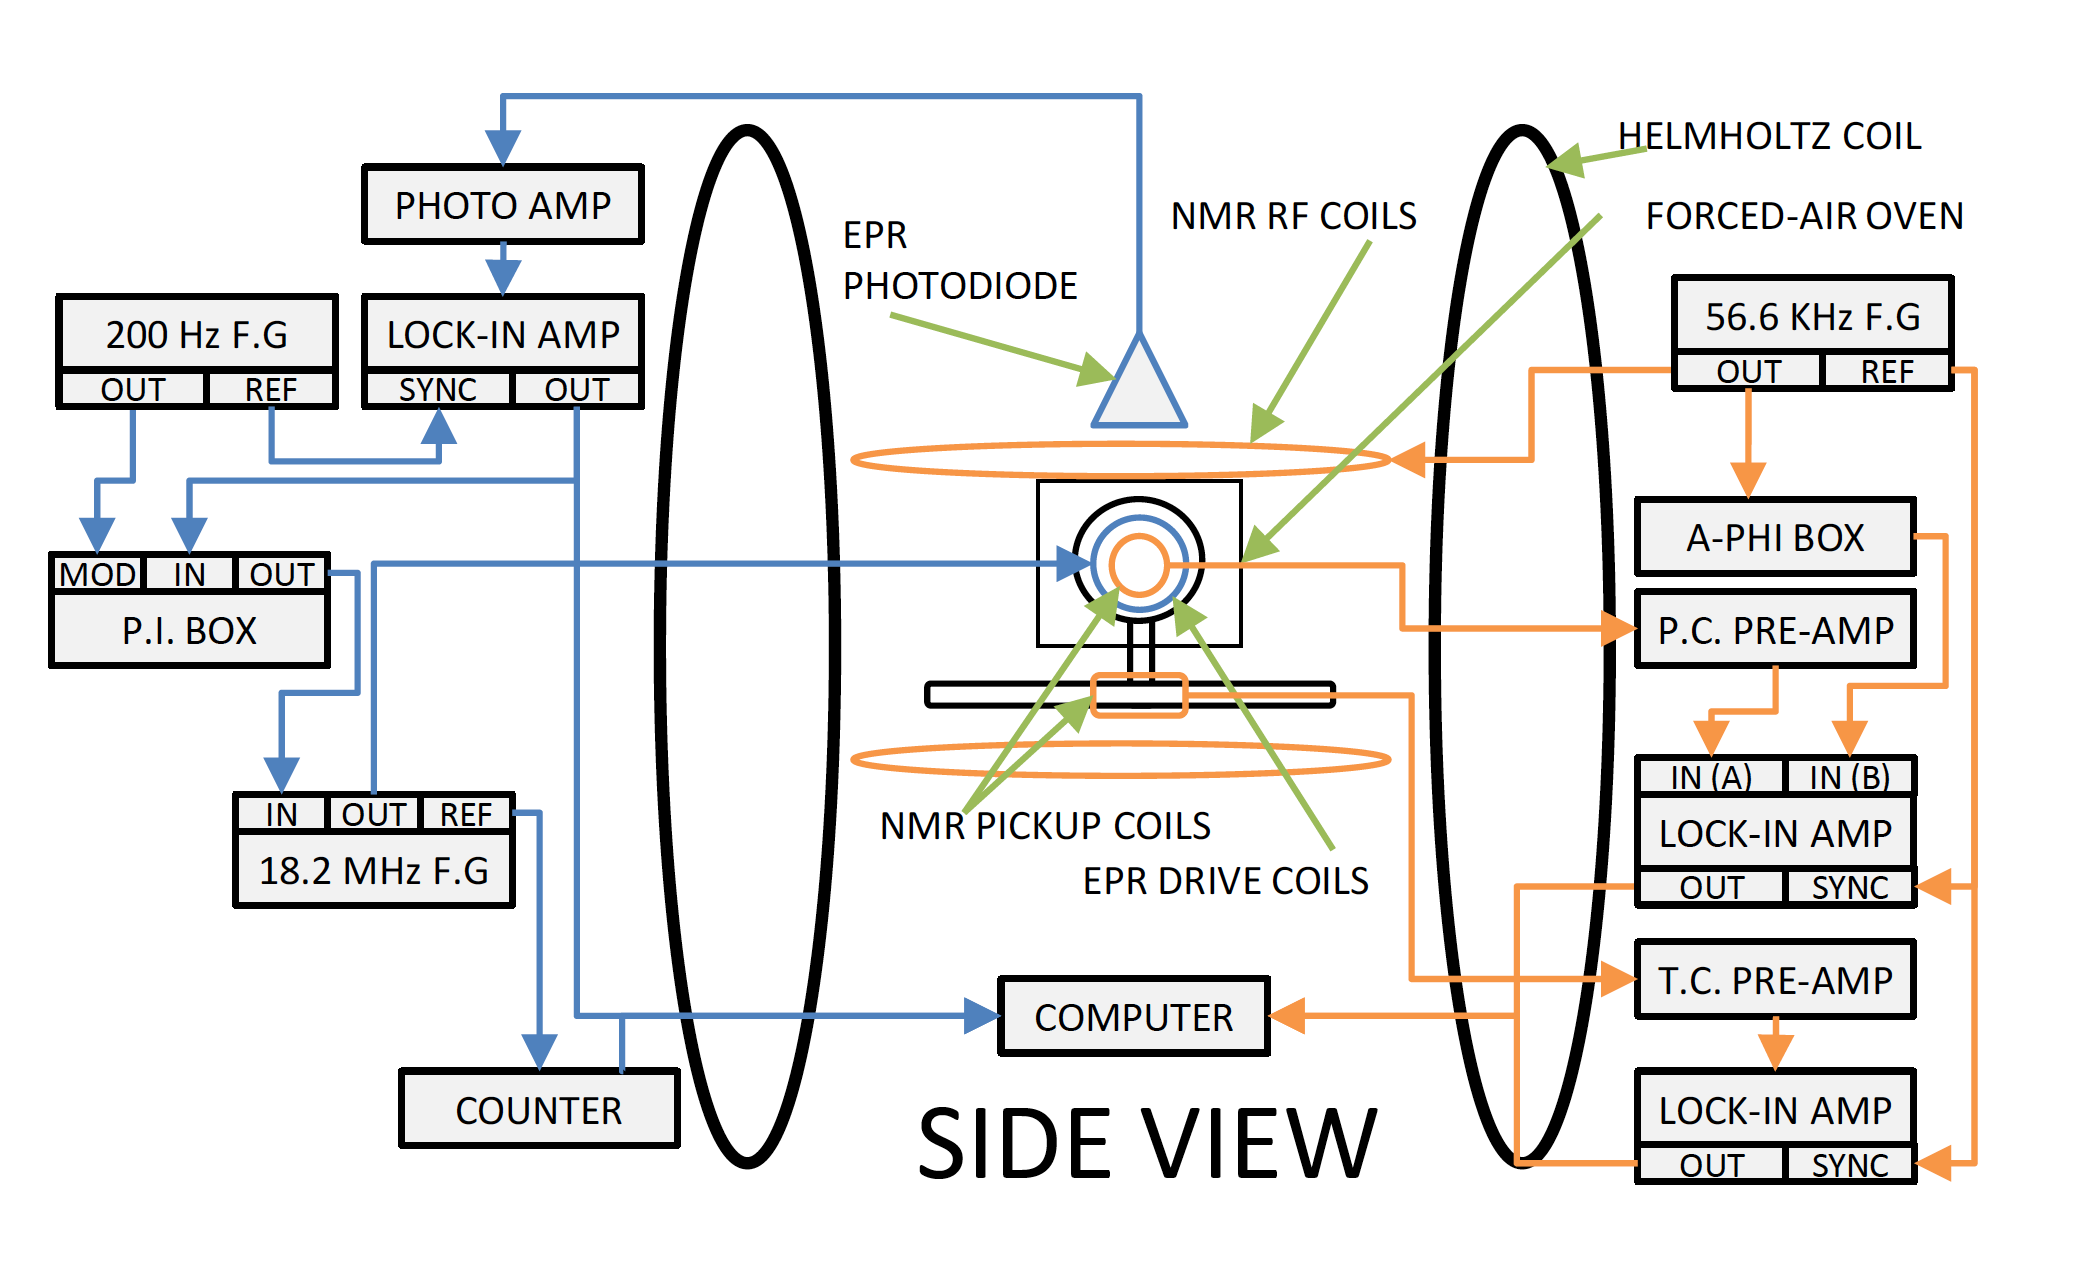
\includegraphics{AFPandEPRsetup.png}}
	\caption{{ EPR (left) and AFP (right) setup. Adapted from Dolph's PhD thesis.}}
	\label{AFPandEPRsetup}
\end{figure}

The flipping process can be achieved by either sweeping the main holding field or sweeping the RF frequency so that the longitudinal component of effective field in the rotating frame goes through zero. AFP measurements in our lab were typically done by sweeping the holding field while keeping the RF frequency constant. The RF coils produced an RF field of magnitude 2$B_{1}$ perpendicular to the main holding field B. The oscillating field has a frequency of $\omega$ and can be decomposed into two counter-rotating components with the same amplitude B$_{1}$. Only the component rotating in the direction able to produce a resonance in Eq.~\ref{EffectiveField} has an important effect. In this frame, the effective field is

\begin{equation}
\vec{B_{eff}}=(B-\omega/\gamma)\vec{z} + B_{1}\vec{x'}
\end{equation}
as discussed above. The other rotating component that rotates in the opposite direction does not affect the spins. In an AFP measurement, the holding field starts from a value lower than $\omega/\gamma$ ($\omega/\gamma-B\gg B_{1}$), so that, initially, the effective field is almost aligned with the holding field and the spins. The holding field is then swept at a constant rate through resonance to a value greater than $\omega/\gamma$. The sweeping rate is of great importance. The sweep needs to be slow enough so that the nuclear spins can follow the effective field

\begin{equation}
\frac{\dot B}{B_{1}}\ll \omega
\end{equation}
Sweep rates that satisfy this condition are considered to be adiabatic.

Sweep rates cannot be too slow either, because the relaxation rate of the spins are faster near the resonance especially with a small effective field B$_{1}$. The relaxation rate of $^{3}$He in the rotating frame due to magnetic field inhomogeneities at resonance is~\cite{PhysRevA.38.5092} 

\begin{equation}
\frac{1}{T_{1r}}=D\frac{|\nabla B_{z}|^{2}}{B_{1}^{2}} 
\end{equation}
where D is the $^{3}$He self-diffusion constant. In order to keep the AFP loss low, it's important for the time scale during which the spins are close to resonance to be much shorter than $T_{1r}$, so we want:

\begin{equation}
D\frac{|\nabla B_{z}|^{2}}{B_{1}^{2}} \ll \frac{\dot B}{B_{1}}
\end{equation}

In the work presented here, the field was typically swept from 12.6 Gauss to 20.4 Gauss in 6s, thus

\begin{subequations}
	\begin{gather}
	\dot B = 1.3G/s\\
	B1 \approx 100mG\\
	f = 56.6kHz\\
	D \approx 0.16cm^2/s\\
	|\nabla B_{z}| \approx 10mG/cm\\
	\end{gather}
\end{subequations}

With these operating conditions, 

\begin{subequations}
	\begin{gather}
	D\frac{|\nabla B_{z}|^{2}}{B_{1}^{2}} \approx 1.6mHz\\
	\frac{\dot B}{B_{1}} \approx 13Hz\\
	\omega \approx 356kHz
	\end{gather}
\end{subequations}

The AFP conditions were clearly well satisfied for our parameters. Fig.\ref{AFP} shows the evolution of effective field in the rotating frame during an AFP measurement.

\begin{figure}[H]
	\centering
	\resizebox{0.91\textwidth}{!}{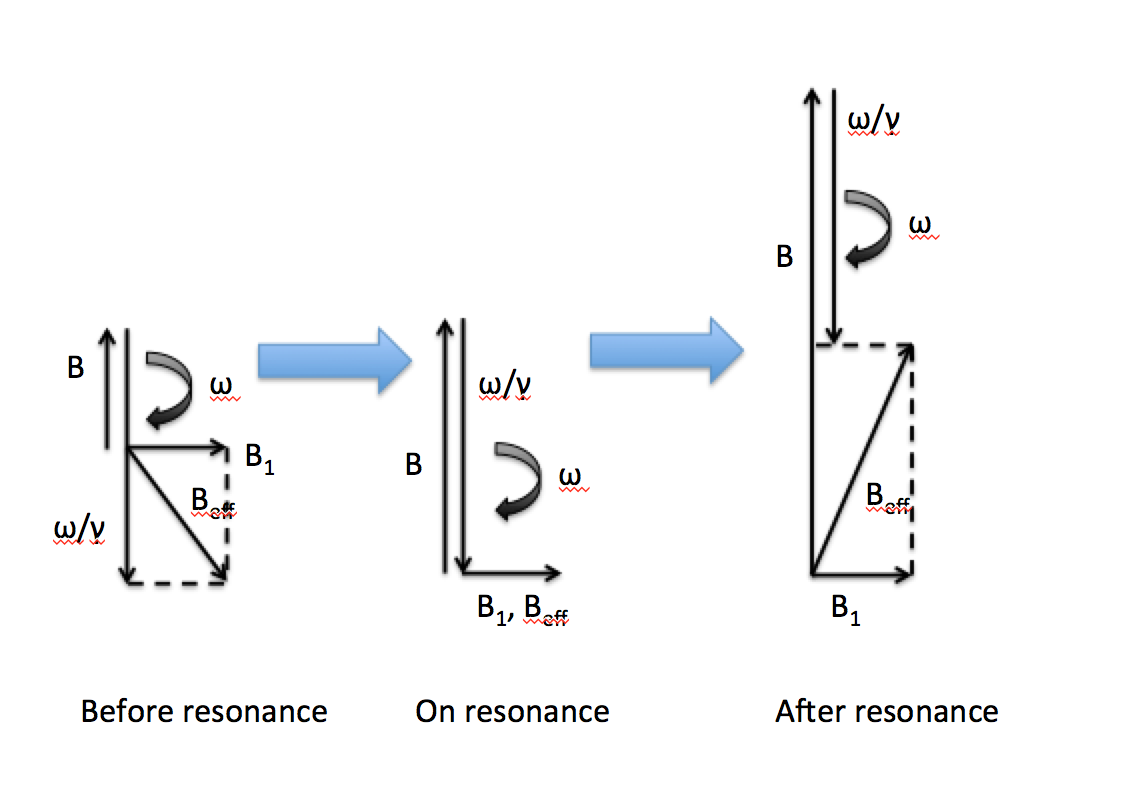
\includegraphics{AFP.png}}
	\caption{{ Effective field in the rotating frame during an Adiabatic Fast Passage measurement. The $^{3}$He spins follow the direction of the effective field. B$_{1}$ is exaggerated to show different components of effective field clearly.}}
	\label{AFP}
\end{figure}

During our AFP measurements, the pick up coils were placed close to the cell, with their axis perpendicular to both the holding field and RF field. Under these conditions, as the $^{3}$He spins precess along the holding field, the transverse component of the spins induces an electromotive force (EMF) that is directly proportional to the amplitude of the component in the pick up coils. The resulting signal can be written as:

\begin{equation}
S=A\omega \sin{\alpha(t)}=A\omega \frac{B_{1}}{\sqrt{B_{1}^{2}+(B(t)-\omega/\gamma)^{2}}}
\end{equation}
where A is a constant that accounts for the cell and coils geometry, the cell magnetization and the electronics factors that affect the size of signal; $\omega$ is the RF frequency; $\alpha$ is the angle between the effective field and the holding field in the rotating frame; B(t) is the holding field as a function of time. The signal reaches peak value when B(t) = $\omega/\gamma$. Fig.\ref{AFPSignal} shows the result of a typical AFP measurement.

\begin{figure}[H]\label{AFPSignal}
	\centering
	\resizebox{0.91\textwidth}{!}{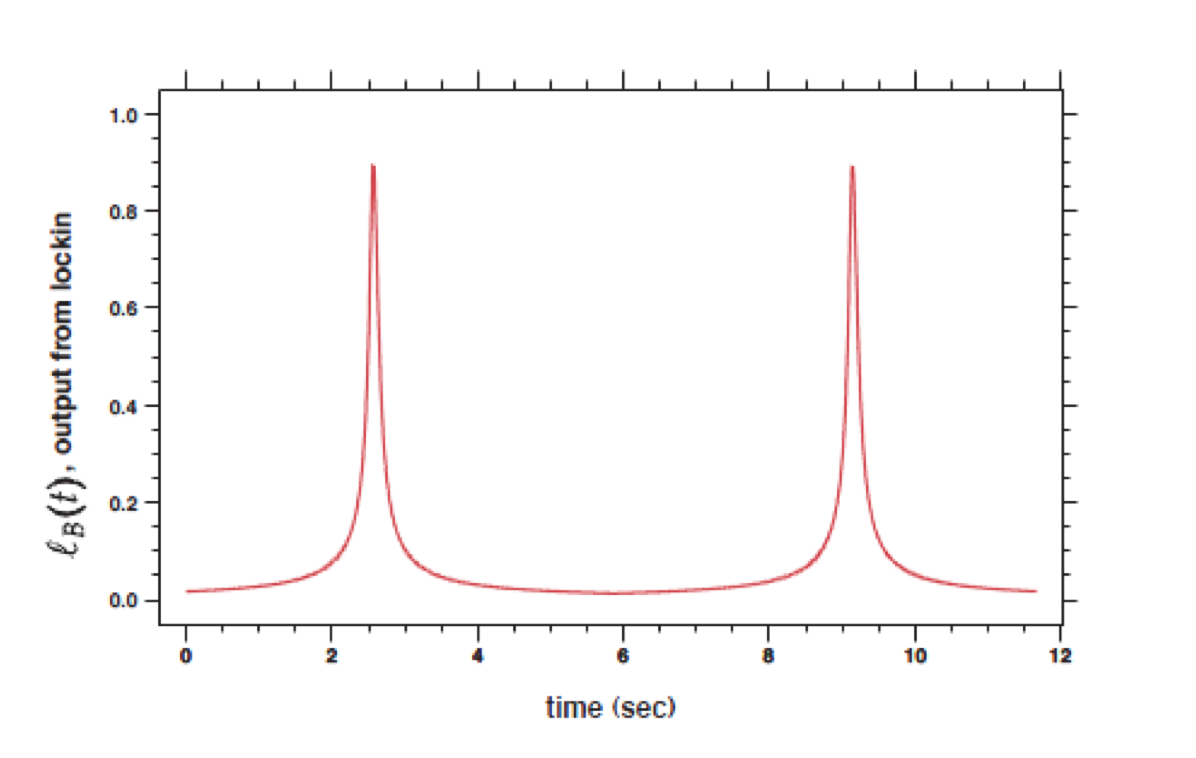
\includegraphics{AFPSignal.png}}
	\caption{{ A typical AFP signal. y axis is in arbitrary unit.}}
	\label{AFPSignal}
\end{figure}

\subsection{AFP Loss}

The longitudinal spin relaxation rate due to static field inhomogeneities is~\cite{PhysRev.138.A946, PhysRev.139.A1398, PhysRevA.37.2877}

\begin{equation}
\frac{1}{T_{1}} = D\frac{|\nabla B_{x}|^{2}+|\nabla B_{y}|^{2}}{B_{0}^{2}}
\end{equation}
where D is the diffusion constant for the polarized spins, and is inversely proportional to the gas pressure. $B_{0}$ is the mean magnetic field along z axis. $B_{x}$ and $B_{y}$ are the x and y components of the magnetic field. However, when performing AFP measurement, the spins are exposed to a small oscillating RF field, the spin relaxation can be greatly accelerated under magnetic resonance conditions~\cite{PhysRevA.38.5092},

\begin{equation}
\frac{1}{T_{r1}} = \frac{8R^{4}}{175D}|\nabla \Omega_{z}|^{2}\sum_{n} \frac{175}{4(\chi_{1n}^{2}-2)(\chi_{1n}^{4}+r^{2}+r^{2}s^{2})(1+s^{2})}
\end{equation}
where R is the cell radius, D is the diffusion constant, $\Omega_{z}$ is the Larmor frequency of the holding field, $r=\frac{\omega_{r}R^{2}}{D}$, $s=\frac{\Omega_{0}-\omega}{\omega_{r}}$, and the numbers $\chi_{1n}$ are the zeros of the derivatives of the spherical Bessel functions

\begin{equation}
\frac{d}{dx}j_{1}(x_{1n})=0~for~n=1,2,3...
\end{equation}

Since $r^{2}\gg \chi_{1n}^{4}$, and $\sum_{n}\frac{1}{\chi_{1n}^{2}-2}=\frac{1}{2}$~\cite{PhysRevA.37.2877},

\begin{equation}
\frac{1}{T_{r1}}=\frac{R^{4}|\nabla\Omega_{z}|^{2}}{r^{2}(1+s^{2})^{2}D}=\frac{|\nabla B_{z}|^{2}D}{B_1^{2}(1+s^{2})^2}
\end{equation}

If $P_{0}$ is the polarization before AFP, the polarization P after a single AFP flip is given by 

\begin{equation}
P=P_{0}e^{-\int \Gamma_{r1} dt}=P_{0}e^{-\int \frac{1}{T_{r1}}dt}
\end{equation}

Thus fraction loss $L_{AFP}$ due to a single AFP flip is:

\begin{equation}
L_{AFP}=1-e^{\int \frac{1}{T_{r1}} dt} \approx \int \frac{1}{T_{r1}} dt
\end{equation}

For our conditions, the integration limits can be extended to $\pm \infty$, making it possible to calculate the integral as:

\begin{equation}
\int_{-\infty}^{\infty} \frac{1}{T_{r1}}dt=\frac{\pi D|\nabla B_{z}|^{2}}{2B_{1}\partial B_{1}/\partial t}
\end{equation}
which is the fractional loss due to a single AFP flip.

To better understand AFP loss, we performed a study where we took AFP measurements at various different field gradients to study the relation between AFP loss and inhomogeneities. The gradients were produced by Maxwell-style transverse gradient coils and increased from 0 to a little under 160 mG/cm. At each set gradient, we take one AFP to look at the difference between the two peaks to determine the loss due to a single flip. Fig~\ref{AFPLossvsGradient} shows AFP losses collected from experiments and theoretical predictions. They agree within the error bar.

\begin{figure}[H]
	\centering
	\resizebox{0.91\textwidth}{!}{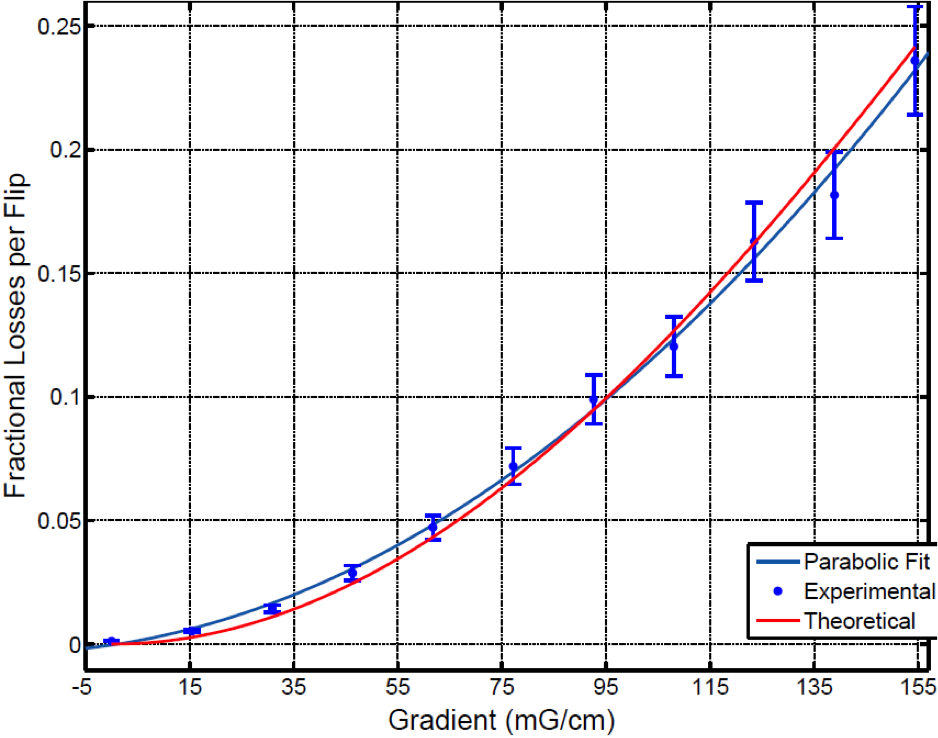
\includegraphics{AFPLossvsGradient.png}}
	\caption{{ Fractional AFP loss (single flip) as a function of field gradient.}}
	\label{AFPLossvsGradient}
\end{figure}

\section{Electron Paramagnetic Resonance}

\subsection{Overview}

Electron Paramagnetic Resonance (EPR) provides an important technique for measuring the frequency shift of alkali metal Zeeman resonances due to the effective magnetic field produced by polarized $^{3}$He gas. During spin-exchange collisions, the alkali valence electron is essentially located within the $^3$He nucleus thus facilitating a Fermi contact interaction between their spins. The EPR shift is largely caused by this Fermi-contact interaction $\alpha$ {\bf K$\cdot$S} between the nuclear spin {\bf K} of the noble gas nucleus of magnetic moment $\mu_{K}$ and the electron spin {\bf S} of the alkali metal atom~\cite{PhysRevA.71.013414}. The magnetic field created by the bulk magnetization of the $^{3}$He gas also contributes directly to a relatively small part of the shift (rougly 1/6 for K). Because the spin-exchange effective field is difficult to calculate accurately from theory, the total measured shift is usually written as the expected Zeeman interaction with the field produced by the polarized $^{3}$He multiplied by an atomic parameter $\kappa_{0}$. The value of $\kappa_0$ can be thought of as an enhancement due to attraction of the alkali electron wave function to the $^3$He nucleus~\cite{PhysRevA.58.3004}, which is different for each alkali metal species and slightly temperature dependent.

During the process of optical pumping, the Rb atoms are excited to the 5P$_{\frac{1}{2}}$ state by the pump laser. The majority of these atoms are quenched non-radiatively to the ground state by N$_{2}$. While in the 5P$_{\frac{1}{2}}$ state, Rb atoms can also be excited to the 5P$_{\frac{3}{2}}$ state through collisions with other Rb atoms. A small fraction of the excited atoms (5P$_{\frac{1}{2}}$ and 5P$_{\frac{3}{2}}$) decay by emitting either a D$_{1}$ photon or D$_{2}$ photon. The intensity of fluorescence is proportional to the population of excited Rb atoms, and is thus higher when the Rb polarization is low so more Rb atoms can absorb laser and jump to the excited state. We typically induce Zeeman transitions with an RF coil to lower alkali polarization and detect D$_{2}$ photons with a photodiode behind a D$_{2}$ filter. The highest amount of D$_{2}$ photons is detected when the RF frequency is exactly equal to the Zeeman transition frequency.

\subsection{The Breit-Rabi Equation}

The Zeeman energy levels of ground state (L = 0) can be described with the Breit-Rabi equation\cite{PhysRev.38.2082.2}

\begin{equation}
E_{F=I\pm 1/2, m_{F}}=-\frac{h\Delta \nu_{hfs}}{2(2I+1)}-\mu_{N}g_{I}Bm_{F}\pm \frac{h\Delta \nu_{hfs}}{2}\sqrt{1+\frac{4m_{F}x}{2I+1} +x^{2}}
\end{equation}
where

\begin{equation}
x=(g_{I}\mu_{N}-g_{s}\mu_{B})\frac{B}{h\Delta \nu_{hfs}}
\end{equation}
B is the magnetic field, $\Delta \nu_{hfs}$ is the hyperfine splitting frequency, I is the nuclear spin, $g_{I}$ and $g_{s}$ are the g factors of nuclear and electron spin, $\mu_{N}$ and $\mu_{B}$ are the nuclear and Bohr magneton, respectively. 

The Zeeman transition frequency of $m_{F} \rightarrow m_{F} - 1$ is 

\begin{equation}
\begin{split}
\nu_{m_{F}\rightarrow m_{F-1}} &=\frac{E_{F,m_{F}}-E_{F,m_{F}-1}}{h} \\
&= -\frac{g_{I}\mu_{N}B}{h}\pm \frac{\Delta \nu_{hfs}}{2}\left(\sqrt{1+\frac{4m_{F}}{2I+1}x+x^{2}}-\sqrt{1+\frac{4m_{F}-1}{2I+1}x+x^{2}}\right)
\end{split}
\end{equation}

The second term is much greater than the first term under our operating conditions, so the sign of the frequency $\nu_{m_{F}\rightarrow m_{F-1}}$ depends on the second term only. If we focus on the $F=I+\frac{1}{2}$ hyperfine manifold, the transition frequency is

\begin{equation}\label{Zeeman}
\nu_{m_{F}\rightarrow m_{F-1}} = -\frac{g_{I}\mu_{N}B}{h}+ \frac{\Delta \nu_{hfs}}{2}\left(\sqrt{1+\frac{4m_{F}}{2I+1}x+x^{2}}-\sqrt{1+\frac{4m_{F}-1}{2I+1}x+x^{2}}\right)
\end{equation}

\subsection{Shift of Zeeman Frequency}

Under our operating condition, the size of Zeeman splitting is much less than hyperfine splitting, which makes x a small number. The Taylor expansion of Eq.~\ref{Zeeman} is

\begin{equation}\label{Taylorwithx}
\begin{split}
\nu_{m_{F}\rightarrow m_{F-1}}=&-\frac{g_{I}\mu_{N}B}{h}\\
&+\frac{\Delta\nu_{hfs}}{2}\left(\frac{2x}{2I+1}-\frac{2(2m_{F}-1)x^{2}}{(2I+1)^{2}}+\frac{(-(2I+1)^{2}+4-12m_{F}+12m_{F}^{2})x^{3}}{(2I+1)^{3}}+\cdots\right)
\end{split}
\end{equation}
with the approximation

\begin{subequations}
	\begin{gather}
	g_{s}\mu_{B} \gg g_{I}\mu_{N}\\
	x \approx -\frac{g_{s}\mu_{B}B}{h\Delta \nu_{hfs}}
	\end{gather}
\end{subequations}
then to the lowest order approximation, the shift of $\nu_{m_{F}\rightarrow m_{F-1}}$ due to a small effective field $\Delta B$ ($\Delta B \ll B$) from polarized $^{3}$He is

\begin{equation}
\begin{split}
\Delta \nu_{m_{F}\rightarrow m_{F-1}} = &-\frac{g_{s}\mu_{B}}{h(2I+1)} \Delta B \left[1+ 2(2m-1)\frac{g_{s}\mu_{B}B}{h \Delta\nu_{hfs}(2I+1)}\right.\\ 
&\left.+6\left(-\frac{(2I+1)^{2}}{4}+1-3m+3m^{2}\right)\left(\frac{g_{s}\mu_{B}B}{h \Delta\nu_{hfs}(2I+1)}\right)^{2}+\cdots\right]
\end{split}
\end{equation}

Usually the pumping chamber is spherical, the magnetic field produced inside a uniformly magnetized sphere is~\cite{Jackson}

\begin{equation}
\Delta \boldsymbol{B}=\frac{2}{3}\mu_{0}\boldsymbol{M}
\end{equation}
where $\mu_{0}$ is the vacuum permeability, $\boldsymbol{M}$ is the magnetization of $^{3}$He, 

\begin{equation}
\boldsymbol{M}=\boldsymbol{\mu_{K}}[{\rm He}]P,
\end{equation}
$\mu_{K}$ is the magnetic moment of $^{3}$He, [He] is its density, and P is its polarization. As we mentioned before, as a result of the Fermi-contact interaction $\alpha${\bf K$\cdot$S} between the nuclear spin {\bf K} of the noble gas nucleus and the electron spin {\bf S} of the alkali metal atom, the effective magnetic field felt by alkali metal due to the polarized $^3$He nuclei is $\kappa_{0}$~\cite{PhysRevA.58.3004}:

\begin{equation}
\boldsymbol{\Delta B}=\frac{2}{3} \kappa_{0}\mu_{0}\boldsymbol{\mu_{K}}[{\rm He}]P
\end{equation}

The enhancement factor $\kappa_{0}$ was measured by Romalis and Cates in 1998 with an error of 1.5\%~\cite{PhysRevA.58.3004}

\begin{equation}
\kappa_{0}^{Rb-^{3}He}=4.52+0.00934[T(^{\circ}C)]
\end{equation}
then it was measured by Babcock~\emph{et al.} in 2005~\cite{PhysRevA.71.013414}

\begin{subequations}
	\begin{gather}
	\kappa_{0}^{Rb}=6.39+0.00914[T-200(^{\circ}C)]\\
	\kappa_{0}^{K}=5.99+0.0086[T-200(^{\circ}C)]\\
	\kappa_{0}^{Na}=4.84+0.00914[T-200(^{\circ}C)]
	\end{gather}
\end{subequations}

The two results agree within the error. Thus we can calculate $^{3}$He polarization with the EPR frequency shift. 

\subsection{Experimental Methods}

\subsubsection{Overview}

Under operating conditions typical when using a polarized $^3$He target, hybrid cells with mixture of Rb and K are used. The vapor density of K is around 6 times as that of Rb, we typically induce the $^{39}$K transition corresponding to $m_{F} = 2 \rightarrow m_{F} = 1$ (assuming the angular momentum of laser photons is +1), which lowers the K polarization. The Rb-K spin-exchange rate is fast enough that the Rb is depolarized almost instantly. This allows more Rb atoms to absorb laser and be excited to the 5P$_{\frac{1}{2}}$ state which in turn produces more D$_{2}$ fluorescence. The D$_{2}$ fluorescence is at maximum intensity when the RF frequency is on resonance for the Zeeman transition. 

We first locate the frequency with a frequency-modulated (FM) sweep, and set the RF frequency to the found value. The RF is locked to the frequency that induces maximum D$_{2}$ light using a proportional-integral feedback circuit (P.I. box). This frequency is referred to as the EPR frequency and is measured with a frequency counter. To separate the frequency-shifting effect of polarized $^{3}$He from other sources that may affect the transition frequency, we flip the $^{3}$He magnetization by performing AFP using an RF frequency sweep. A frequency sweep is chosen rather than a holding field sweep  to keep external magnetic field constant, thus reducing factors that affect Zeeman splitting size. No signal is recorded during theses sweeps, as the varying frequency would affect the amplitude of AFP signals. By comparing the frequency measured before and after the flip, together with the real temperature inside the pumping chamber, we can calculate the $^{3}$He polarization. We typically take AFP measurements (in our usual way using a magnetic field sweep) right before and after the relatively quick EPR measurement, so that a calibration constant that translates AFP signal size to $^{3}$He polarization can be calculated.

\subsubsection{Locating Zeeman Transition Frequency}

The P.I. box only works well in locking the EPR frequency to the $m_{F}=2\rightarrow m_{F}=1$ K transition when the EPR frequency is close to the transition. Thus, the first step in EPR measurements is to locate the Zeeman transition. A frequency-modulated (FM) sweep is performed through a range that covers the Zeeman transition, the range is known from experience or calculation and the P.I. box remains off during the sweep.

The RF frequency is generated by a voltage-controlled oscillator (VCO). The D$_{2}$ fluorescence is detected with the photodiode and recorded during the sweep. The RF is frequency-modulated by a 200Hz signal, and the VCO output at any moment during the sweep can be described as: 

\begin{equation}
V_{FM}(t)=V_{C0}\sin{\left(2\pi[f_{c}+D_{f}\sin{\left(2\pi f_{m}t+\phi_{m}\right)}]t+\phi_{c}\right)}
\end{equation}
where $V_{C0}$ is the amplitude of the sweeping RF frequency (carrier), $f_{c}$ is the RF frequency that is being swept through a set range, $D_{f}$ is the peak frequency deviation, $f_{m}$ is the modulating frequency (200Hz in our case), and $\phi_{m}$ and $\phi_{c}$ are the phase of the modulation frequency and carrier frequency, respectively. Thus, the RF frequency is

\begin{equation}
f_{FM}(t) = f_{c}(t)+D_{f}\sin{\left(2\pi f_{m}t+\phi_{m}\right)}
\end{equation}
where $f_{c}(t)$ emphasizes the RF frequency is sweeping over time. 

The D$_{2}$ light intensity can be described with a Lorentzian function:

\begin{equation}\label{D2light}
I(f(t))=\frac{I_{0}}{(f_{FM}(t)-f_{0})^{2}+\Gamma^{2}}
\end{equation}
where $f_{0}$ is the Zeeman transition frequency, $\Gamma$ is the line width. Keeping the first order term of the Taylor expansion of Eq.~\ref{D2light}, the D$_{2}$ light intensity is

\begin{equation}
I(f(t))=I(f_{c}(t))+\frac{\partial I}{\partial f}\Bigm|_{f=f_{c}(t)}D_{f}\sin{\left(2\pi f_{m}t+\phi_{m}\right)}
\end{equation}

A lock-in amplifier is used to select only the $f_{m}$ term to reduce the noise, which is proportional to the derivative of the Lorentzian function multiplied by a sine function. The FM sweep line crosses zero when the RF frequency is equal to the Zeeman transition frequency (peak of the Lorentzian function), which produces the maximum D$_{2}$ light intensity. The region between the lowest and highest points of the derivative line is fitted to a line, and the zero-crossing point of the line is used as the Zeeman transition frequency. Fig.~\ref{fmsweep} shows an FM sweep.

\begin{figure}[t!]
	\centering
	\resizebox{0.91\textwidth}{!}{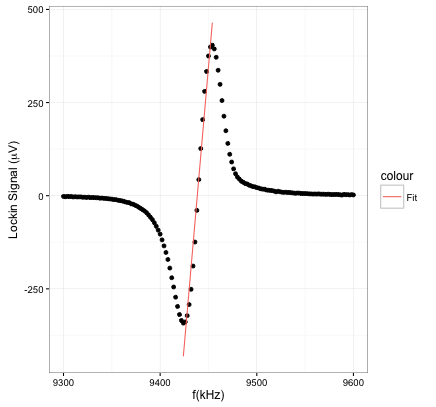
\includegraphics{fmsweep.png}}
	\caption{{ A typical FM sweep on a hybrid cell. The central region between the minimum and maximum is fitted to a line. The zero crossing point corresponds to the Zeeman transition frequency.}}
	\label{fmsweep}
\end{figure}

\subsubsection{EPR Spin Flip Process}

After the transition frequency is located, the VCO frequency is first set to it and then locked with a proportional-integral feedback circuit (P.I. box). The circuit is shown in Fig.~\ref{PIBox}. 

\begin{figure}[t!]
	\centering
	\resizebox{0.91\textwidth}{!}{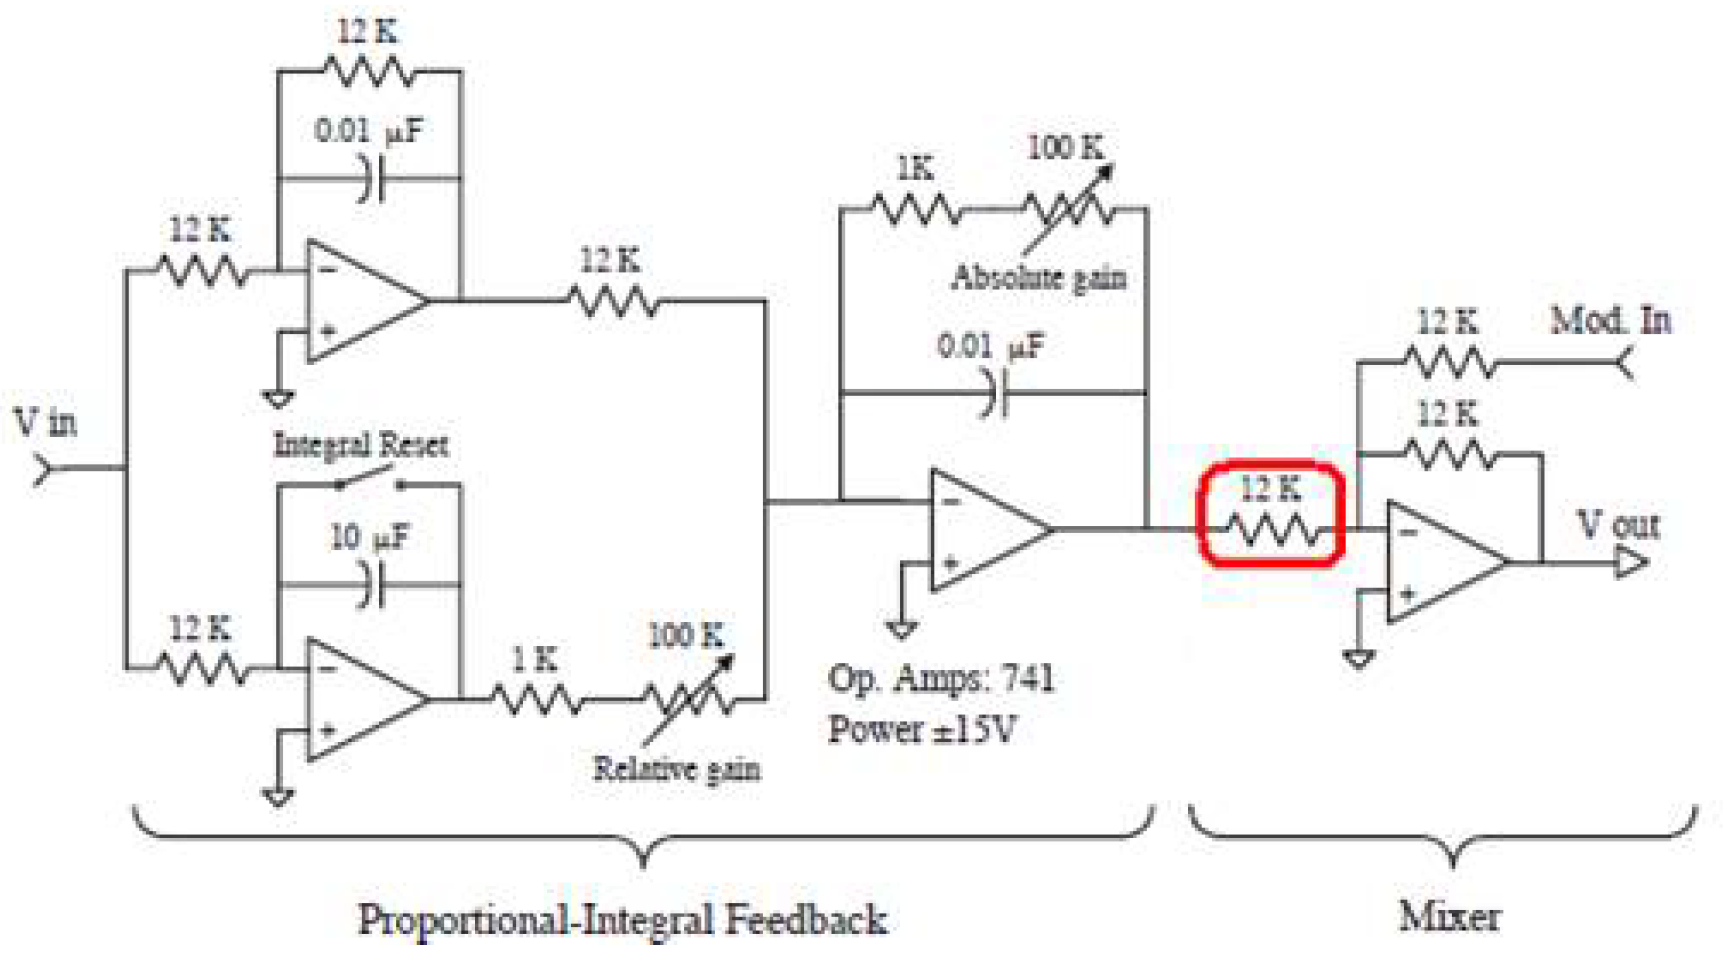
\includegraphics{PIBox.png}}
	\caption{{ The same P.I. circuit that was first used by Romalis in our lab. The drawing was then corrected by Peter Dolph.\cite{PeterThesis}}}
	\label{PIBox}
\end{figure}

The output of the lock-in amplifier serves as an error signal and the input to the P.I. box. The output of the P.I. box is thus forced to a condition that minimizes the error signal and keeps the VCO centered on the resonant frequency.

Because the EPR frequency is also affected by sources other than the polarized $^{3}$He such as the holding field and earth field, we flip the $^{3}$He spins by sweeping the frequency while keeping the holding field unchanged. The contribution from the flipped spins has the opposite sign while other factors still contribute in the same way, which allows us to extract the change of Zeeman transition frequency due to polarized $^{3}$He, and consequently, calculate the polarization. We typically let the cell polarization reach saturation before performing EPR measurements. AFP measurements are taken right before and after the EPR measurements for calculating the calibration constant (the ratio between polarization and AFP signal size). Fig.~\ref{epr} shows a typical EPR spin flip process.

\begin{figure}[t!]
	\centering
	\resizebox{0.91\textwidth}{!}{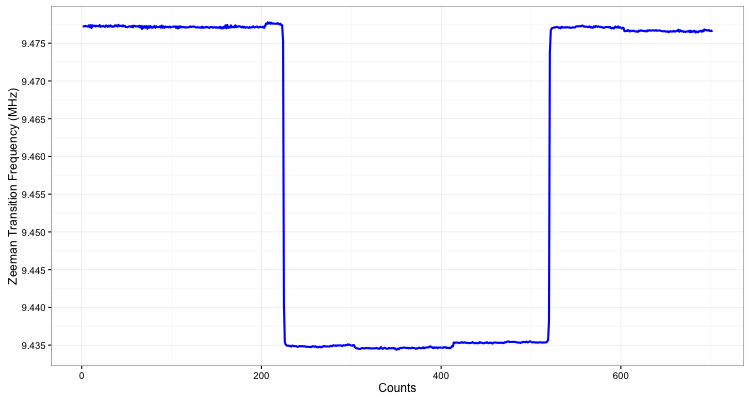
\includegraphics{epr.png}}
	\caption{{ An EPR measurement for a hybrid cell at 235$^{\circ}$C.}} The spins are flipped around 200 mark, and flipped back around 500 mark.
	\label{epr}
\end{figure}

Under normal operating conditions for a double-chambered cell, the pumping chamber is heated to around 170$^{\circ}$C or 235$^{\circ}$C depending on if the cell is hybrid, while the target chamber and transfer tube remain at room temperature. The temperature difference causes differences in gas densities and affects the AFP signal size. The temperature controller of the oven only maintains the surface temperature of the pumping chamber at a set temperature, but the gas inside the pumping chamber is always hotter due to absorption of laser energy. The enhancement factor $\kappa_{0}$ is also slightly temperature dependent which may be underestimated by $\sim$4\% when using the surface temperature as the gas temperature. Dolph described a method we referred to as a ``temperature test" to extract gas temperature inside the pumping chamber in detail in his thesis~\cite{PeterThesis}. In a temperature test, we take AFP measurements when the laser is blocked and unblocked multiple times. With the assumptions that the change of gas densities due to absorption of laser and AFP losses are the only reasons for the difference in signal size, and the temperature measured by RTDs on the exterior of the pumping chamber truly reflects the gas temperature when laser is blocked, one can calculate the inside temperature when laser is unblocked. 

\section{Pulsed Nuclear Magnetic Resonance} 

Adiabatic Fast Passage has been the main technique used in our lab for monitoring relative $^{3}$He polarization during various studies. In an AFP measurement, all $^{3}$He spins are flipped by sweeping the holding field while applying an RF field. As discussed by Chapter 5, we have been exploring the possibility of replacing conventional glass windows with metal end windows for future experiments planned during the 12 GeV era. Because of the lack of studies on spin relaxation of polarized $^{3}$He on metal surfaces, various test cells made with large metal parts as well as glass parts are being studied in our lab. The inclusion of metal parts immediately renders AFP almost useless because of effects such as Eddy currents. Thus, we have been using Pulsed Nuclear Magnetic Resonance (PNMR) for monitoring polarization when studying cells that include metal parts.

\subsection{The Rotating Coordinate System}

In a PNMR measurement, a short pulse of RF frequency is applied to a small localized portion of $^{3}$He gas. The RF frequency is tuned to be on resonance at the Larmor frequency of the holding field. As discussed before with AFP, in the rotating coordinate system, there will be an effective field due to rotation that exactly cancels the holding field which we assume to be in the z direction. Thus the z component of the effective field is zero and there is a non-zero constant transverse component which we will call B$_{1}$. The nuclear spins will precess along B$_{1}$ and end up at an angle away from z axis: 

\begin{equation}
\alpha = \gamma B_{1} \Delta t
\end{equation}
where $\alpha$ is the angle (tip angle), $\gamma$ is the gyromagnetic ratio, and $\Delta t$ is the RF pulse duration. 

\subsection{Free Induction Decay}

At the end of the RF pulse, the tipped spins will have a transverse component equal to the magnetization multiplied by $\sin{\alpha}$. The spins continue to precess along the holding field and the transverse component will induce a signal in the pickup coils (wrapped around the transfer tube as shown in Fig.~\ref{PNMR_setup}) whose axis is perpendicular to the holding field.  

\begin{figure}[t!]
	\centering
	\resizebox{0.91\textwidth}{!}{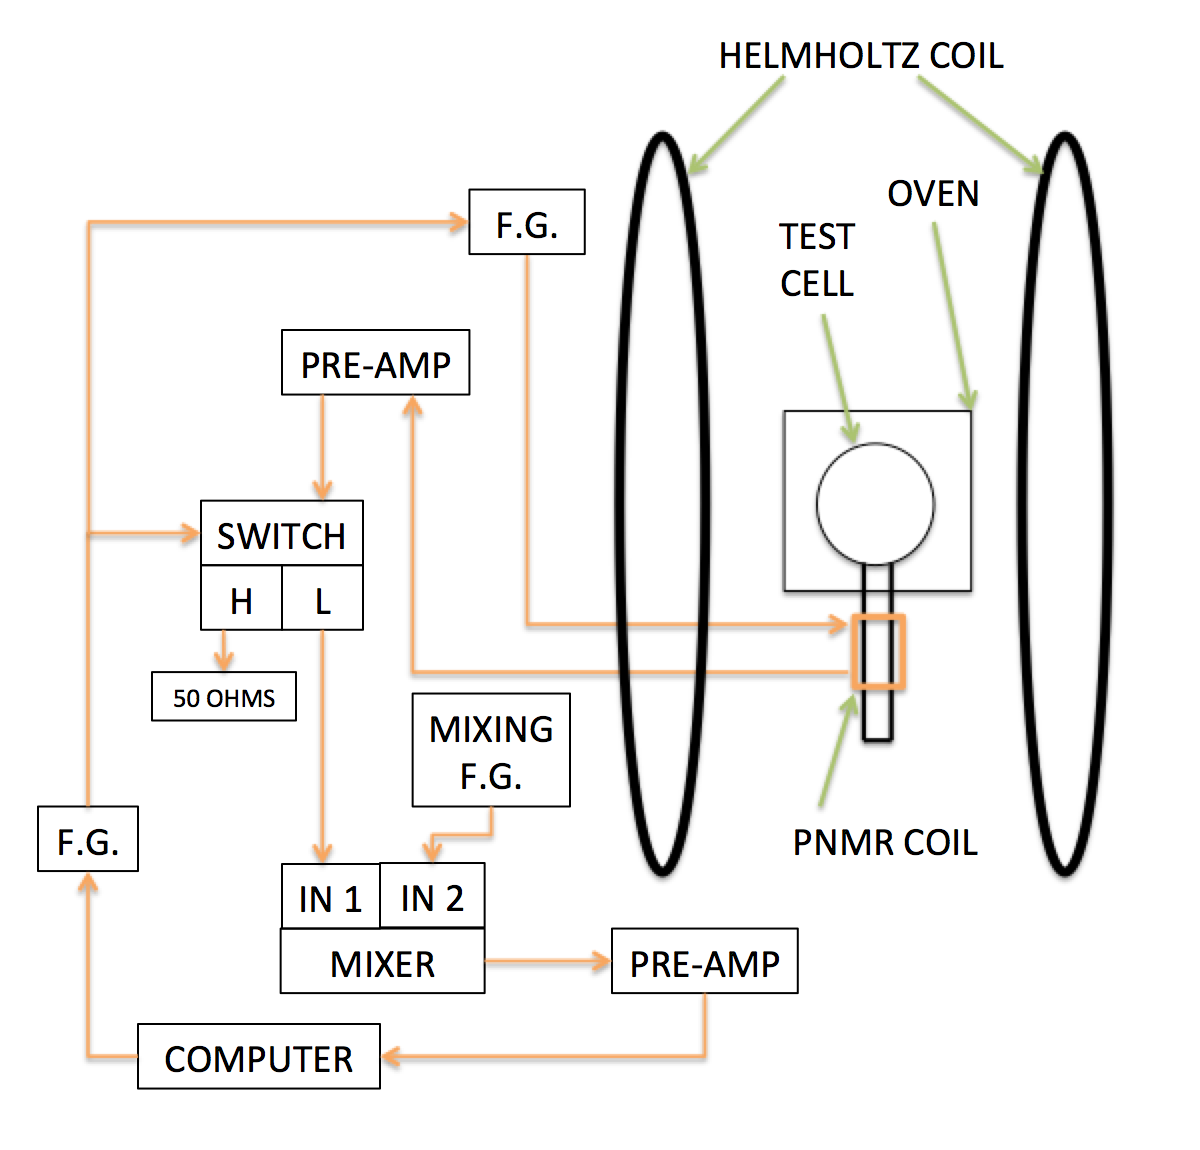
\includegraphics{PNMR_setup.png}}
	\caption{{ PNMR setup.}}
	\label{PNMR_setup}
\end{figure}

In addition to precession, the spins are affected by two types of relaxation processes. The first type is called the spin-lattice relaxation, it describes the rate at which the longitudinal component of magnetization approaches the thermodynamic equilibrium value. It is characterized by the spin-lattice relaxation time constant T$_{1}$. The rate of change of the longitudinal component is

\begin{equation}
\dot{M_{z}}=-(M_{z}-M_{0})/T_{1}
\end{equation}
where M$_{0}$ is the thermodynamic equilibrium magnetization. Solving the differential equation gives

\begin{equation}
M_{z}(t)=M_{0}-\left[M_{0}-M_{z}(0)\right]e^{-t/T_{1}}
\end{equation}

The name spin-lattice relaxation refers to the process in which the spins transfer energy to surrounding, thereby restoring their equilibrium state.

The second relaxation process is relaxation in the transverse plane, which is also referred to as the T$_{2}$ relaxation and was historically called ``spin-spin relaxation". The transverse component of magnetization decays because random fluctuations of the holding field cause different moments to precess at different rates. This is the T$_{2}$ process. Normally, the dominating relaxation effect however, is another dephasing process due to holding field inhomogeneities over the volume of the cell. 

The measured transverse relaxation rate of the tipped spins is the result of all these effects combined:

\begin{equation}
\frac{1}{T_{2}^{*}}=\frac{1}{T_{2}}+\gamma \Delta B_{0}
\end{equation}
where $\Delta B_{0}$ is the variation in the holding field. $\gamma \Delta B_{0}$, the dominant term, is a spread in Larmor frequencies $\Delta \omega_{0}$, which causes spin-spin dephasing in a characteristic time of $1/\Delta \omega_{0}$. 

The time evolution of the nuclear magnetization {\bf M} can be described by the Bloch equations~\cite{PhysRev.70.460}:

\begin{subequations}
	\begin{gather}
	\frac{\partial M_{x}(t)}{\partial t}=\gamma\left(\boldsymbol{M(t)}\times \boldsymbol{B(t)}\right)_{x}-\frac{M_{x}(t)}{T_{2}^{*}}\\
	\frac{\partial M_{y}(t)}{\partial t}=\gamma\left(\boldsymbol{M(t)}\times \boldsymbol{B(t)}\right)_{y}-\frac{M_{y}(t)}{T_{2}^{*}}\\
	\frac{\partial M_{z}(t)}{\partial t}=\gamma\left(\boldsymbol{M(t)}\times \boldsymbol{B(t)}\right)_{z}-\frac{M_{z}(t)}{T_{1}}
	\end{gather}
\end{subequations}
where $\gamma$ is the gyromagnetic ratio and the cross products are the precession terms, the last terms in each equation represent the decaying and dephasing of each component. The precessing spin magnetization generates a signal in the pickup coils that decays with time. This is called free induction decay, the induced signal is typically described by

\begin{equation}
V(t)=A\omega_{0}\sin{\alpha}\sin{\left(\omega_{0}t+\phi\right)}e^{-t/T_{2}^{*}}
\end{equation}
where A is just a constant, $\omega_{0}$ is the Larmor frequency for the holding field, $\alpha$ is the tip angle, T$_{2}^{*}$ is the measured decay time constant. For our metal test cells, depending on the location of the pickup coils and the field setup, T$_{2}^{*}$ varies between several milliseconds to more than 300 milliseconds.

\subsection{Experimental Methods}

Our PNMR setup is shown in Fig.~\ref{PNMR_setup}. The Labview program on the computer controlled the timing of a gate signal that was fired from the first function generator (F.G.). The gate signal was fed to the back of the second function generator and triggered it to produce a short pulse. The second function generator sent out RF pulse with pre-set amplitude, duration and frequency only when the gate signal was of voltage higher than the threshold. The frequency of the RF pulse was carefully tuned to be at the Larmor frequency of the holding field. 

The pulse was sent from the function generator to a coil wrapped directly on a small portion of the cell. The spins in the proximity of the coil were exposed to the pulse and tipped by an angle which depended on the amplitude and the duration of the pulse. In the rotating frame, the effective field B$_{1}$ caused the spins to precess around it (as discussed before), the precession frequency was $\gamma B_{1}$ so the angle the spins rotate by (tip angle) can be calculated by:  

\begin{equation}\label{tip_angle}
\alpha = \gamma B_{1} \Delta t
\end{equation}
where $\gamma$ is the gyromagnetic ratio, the effective field B$_{1}$ is directly proportional to the amplitude of the RF pulse, and $\Delta$t is the duration of the pulse. Ideally, a 90$^{\circ}$ tip angle would result in the maximum signal, but it had not been the case for us most of the time. The coils were normally wrapped on the transfer tube of the cell which was off the center of the holding field and exposed to relatively large holding field inhomogeneities. Different groups of spins contributed to the FID signal also saw different values of $B_1$. The details of how we measure the test cells will be discussed in later chapters. As a result, the spins to precessed at different rates, and the dephasing became more significant with longer pulse duration and larger tip angle, which led to non-optimal signals. Exact tip angles of specific group of spins depended on location, a typical effective tip angle for the whole region would be between 30$^{\circ}$ and 45$^{\circ}$. 

After the spins were tipped away from z axis, they precessed around the holding field and induced a signal in the detection coil. The signal was amplified by a low noise pre-amplifier first and then went through an isolation switch. The switch only let signal pass when the controlling gate voltage was low, thus stopped the RF pulse from coming back through the detection circuit. The signal was at the Larmor frequency, and was mixed with another frequency after the switch. The mixing frequency was only slightly different from the Larmor frequency, the output of the mixer had both the sum of the two frequencies and the difference. A second pre-amplifier was used to select and amplify the lower of the two frequencies while filtering out high frequency noises. The final output was displayed on a oscilloscope and collected by the Labview program on the computer. Fig.~\ref{FID} shows a PNMR measurement with around 150 ms decay time constant.

\begin{figure}[H]
	\centering
	\resizebox{0.91\textwidth}{!}{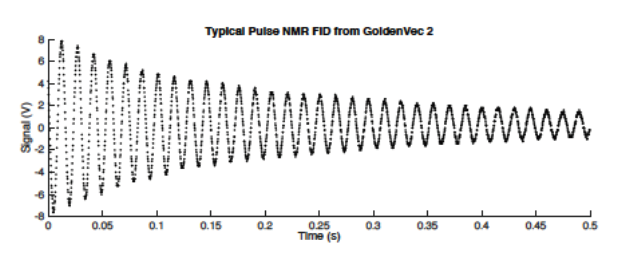
\includegraphics{FID.png}}
	\caption{{ A PNMR signal taken with gold coated test cell.}}
	\label{FID}
\end{figure}

The tip angle was measured with a short sequence of FID signals. Theoretically the tip angle can be calculated with Eq.~\ref{tip_angle}. But because of inhomogeneities and other factors, the calculation serves as only an estimate in practice and it was often more accurate and convenient to measure the tip angle directly. We took several PNMR measurements in quick succession with the same RF pulse settings. After every pulse, the transverse component of the spins quickly decayed and dephased, leaving only the longitudinal component which was equal to $\cos{\alpha}$ times the original magnetization. The intervals between measurements were short enough so that T$_{1}$ can be safely ignored. The series of measurements also needed to be performed on the same portion of the gas (i.e. the same group of spins tipped by the first pulse), thus it was important to know that the self-diffusion of $^{3}$He was significantly slower than the sampling rate. The self-diffusion coefficient of $^{3}$He at 300K is~\cite{J.Phys.France.35}

\begin{equation}
D=\frac{1440(80){\rm torr}}{{\rm P}}{\rm cm^{2}/s}
\end{equation}
which is roughly 1.89 cm$^{2}$/s at 760 torr (the test cells normally contained around 1 atm of $^{3}$He). The diffusion length is described by

\begin{equation}
l = 2\sqrt{Dt}
\end{equation}

Thus in one second, the gas moved around 2.75 cm through self-diffusion. For this reason, we only took 2 or 3 PNMR measurements to calculate the tip angle. As additional measurements would have given enough time for the tipped spins from the first PNMR and the surrounding spins to mix.

Since only the longitudinal component of the tipped spins were preserved, the amplitude of the i$_{th}$ PNMR was

\begin{equation}
V_{i}=V_{0}cos^{i-1}\alpha 
\end{equation}
where V$_{0}$ is the induced signal in the first PNMR. We could then use this equation to calculate the effective tip angle $\alpha$.






